%
% File main.tex
%
% NLP course final-report-structure template, Warsaw University of Technology.
% Prepared by Anna Wróblewska, adapted from the ACL 2015 conference
% formatting template (acl2015.sty), originally by the ACL 2015
% organizers and earlier ACL/EACL format authors (see acl2015.pdf
% for the full credits chain).

\documentclass[11pt]{article}
\usepackage{acl2015}
\usepackage{times}
\usepackage{caption}
\usepackage{url}
\usepackage{latexsym}
\usepackage[T1]{fontenc}
\usepackage{xcolor}
\usepackage{amsmath,amssymb}
\usepackage{booktabs, tabularx}
\usepackage{tikz}
\usepackage{hyperref}
\usetikzlibrary{arrows.meta,positioning}
\usepackage{array,booktabs,ragged2e}
\newcolumntype{P}[1]{>{\RaggedRight\arraybackslash}p{#1}}
\newlength{\annotationwidth}
%\setlength\titlebox{5cm}
\usepackage{float}

\makeatletter
\renewenvironment{thebibliography}[1]
  {\section*{References}
   \list{[\arabic{enumi}]}{%
     \settowidth{\labelwidth}{[#1]}%
     \setlength{\leftmargin}{\labelwidth}%
     \addtolength{\leftmargin}{\labelsep}%
     \usecounter{enumi}%
   }%
   \def\newblock{\hskip .11em plus .33em minus .07em}%
   \sloppy
  }
  {\endlist}
\makeatother

\title{
Is LLM self-consistency a usable signal for routing annotation work?
Phase-1 Raport: Literature overview and concept.}
% https://www.overleaf.com/project/63440c16442dba647b52a1ae
\author{Mikołaj Twardowski \\
  320585 \\
  {\tt 01171182@pw.edu.pl} \\
  \And
  Aleksandra Idczak \\
  327185 \\
  {\tt 01180604@pw.edu.pl} \\
  \And
  Kacper Wnęk \\
  320669 \\
  {\tt 01171276@pw.edu.pl} \\
  }

\date{}
\begin{document}
\maketitle


\begin{abstract}
Large language models can reduce manual annotation costs, but reliable allocation of work between models and humans requires confidence signals that predict annotation correctness. This project investigates whether self-consistency, defined as agreement across repeated model outputs, provides such a signal for Polish multi-label annotation of persuasion and manipulation techniques. Although consistency-based annotation has shown promise in other settings, repeated agreement may reinforce systematic errors, particularly for rare labels and predominantly negative decisions. We propose an evaluation of Bielik-11B-v3.0, PLLuM-12B and Gemma-3-12B-it on the Polish subset of SemEval-2023 Task 3 and MIPD. Self-consistency will be compared with decision-token log-probability, verbalised confidence and additional baselines against human gold labels.  The deliverables will include a reproducible comparison of confidence signals and routing curves relating annotation quality to estimated human workload. 
\end{abstract}

\section{Introduction}

\noindent\textbf{Background.}
Manual text annotation requires time, domain knowledge
and consistent application of annotation guidelines,
making it costly to scale. Identifying persuasion and
manipulation techniques is particularly demanding because
labels depend on context and multiple techniques may
co-occur. Large language models (LLMs) offer a way to
reduce this workload by assigning labels from natural-language
instructions. However, their errors motivate human--LLM
collaboration, in which selected model annotations are
accepted automatically and others receive human review
\cite{coannotating-uncertainty}.

\smallskip
\noindent\textbf{Problem statement.}
The central question is whether agreement across repeated
LLM outputs predicts label correctness well enough to
support this allocation. We define self-consistency as
the proportion of sampled outputs supporting the majority
decision for an item--label pair. Agreement does not
guarantee correctness: repeated outputs may reproduce
the same error. Although consistency-based annotation
has been demonstrated for factual claim detection
\cite{afacta-assist}, its usefulness relative to other
confidence signals requires evaluation in our setting:
Polish multi-label detection of persuasion and manipulation
techniques. Rare labels and frequent negative decisions
make aggregate agreement insufficient to establish
reliable annotation.

\smallskip
\noindent\textbf{Project contributions.}
We will compare self-consistency with decision-token
log-probability, verbalised confidence and random routing
using three instruction-tuned models on Polish
SemEval-2023 Task~3 and MIPD
\cite{2023-semeval,mipd-2024}.
The planned contributions are:
(1) an evaluation of how consistency predicts correctness
across models, datasets and individual labels;
(2) an analysis of within-prompt sampling variability and
differences across prompt configurations;
(3) routing curves relating annotation quality to estimated
human workload, with thresholds selected on separate
calibration data.

\section{Related Work and State of the Art}

\noindent\textbf{LLMs as annotators.}
Early studies established the potential of model-generated
labels. GPT-3 can reduce the cost of producing training
annotations \cite{want-to-reduce-gpt3}, while ChatGPT
outperforms crowd workers on selected relevance, stance,
topic and framing tasks
\cite{chat-gpt-outperform-crowd}.
However, evaluations across non-public social-science
datasets identify uneven performance
\cite{keeping-humans-annot}, and task-specific comparisons
show that strong results do not generalise uniformly
\cite{are-chatbots-reliab}.
The practical challenge is therefore identifying which
individual labels can be accepted reliably.

\smallskip
\noindent\textbf{Confidence and selective annotation.}
CoAnnotating uses uncertainty to allocate annotation
between humans and LLMs, evaluating the resulting labels
through downstream classifier performance
\cite{coannotating-uncertainty}.
AFaCTA uses agreement across three predefined reasoning
paths to identify reliable factual-claim annotations
\cite{afacta-assist}.
More broadly, confidence-elicitation research compares
verbalised confidence with consistency across sampled
answers \cite{can-llm-expre}.
These approaches establish uncertainty-guided annotation
as a relevant baseline, rather than a new contribution
of this project.

\smallskip
\noindent\textbf{Position of this project.}
We extend this line of evaluation to Polish multi-label
technique annotation, comparing confidence signals
directly against human gold labels.
Unlike downstream-classifier evaluation, this isolates
annotation correctness and its usefulness for routing.
We additionally examine rare-label errors and translate
decision-level deferral into item-level review workload.
Table~\ref{tab:annotation} summarises the reviewed studies.



\begin{table*}[t!]
\centering
\fontsize{7}{7.5}\selectfont
\setlength{\tabcolsep}{2pt}
\setlength{\parskip}{0pt}
\renewcommand{\arraystretch}{0.95}
\begin{tabular}{@{}P{0.19\textwidth} P{0.19\textwidth} P{0.13\textwidth} P{0.17\textwidth} P{0.25\textwidth}@{}}
\toprule
\textbf{Work} & \textbf{What it does} & \textbf{Data} & \textbf{Split} & \textbf{Results}\\
\midrule
\textit{Keeping Humans in the Loop: Human-Centered Automated Annotation with Generative AI} \cite{keeping-humans-annot} & GPT-4 replicates human annotation. They compare its predictions with human labels, refine the instructions based on recurring errors. & 27 tasks, 11 non-public social-science datasets; $\sim$75,000 samples annotated & source-document; 250 random human-labelled samples for prompt tuning, 1,000 held-out per task. & 
median accuracy of 0.850.

median F1 of 0.707.

Nine of the 27 tasks were below 0.5 on precision or recall.\\



\textit{MIPD: Exploring Manipulation and Intention In a Novel Corpus of Polish Disinformation} \cite{mipd-2024} & Evaluates GPT-4 and GPT-3.5 for zero-shot binary disinformation classification, with and without a definition in the prompt. & MIPD: 15,356 Polish articles; 10,359 credible, 4,997 disinformative & article; random 10\% evaluation sample ($\approx$1,536 articles; & weighted F1 (without/with definition): GPT-4 0.84/0.86;

GPT-3.5 0.61/0.70
\\


\textit{Evaluating Decision Models for Text Annotation in Computational Social Science} \cite{eval-decis-2026} (preprint) & Zero-shot comparison of a decision model (typed label choice plus confidence) with 19 LLMs; items are routed by confidence and low-confidence ones escalated to a stronger LLM. & 18 CSS classification tasks, 7,977 items ($\leq$500 per task) & utterance / conversation / document; released test splits, class-stratified sample &
At confidence $\geq 0.9$, median accuracy / coverage(how many examples got that high confidence)
across 15 evaluation tasks:

Opus 5: 86.2\% / 25.9\%;

Fable 5.1: 95.3\% / 19.2\%;

Sonnet 5: 94.2\% / 9.5\%.



\\


\textit{ChatGPT Outperforms Crowd-Workers for Text-Annotation Tasks} \cite{chat-gpt-outperform-crowd} & Evaluates zero-shot ChatGPT annotation of relevance, stance, topics and frames against trained annotators and MTurk workers. & 6,183 texts:content-moderation tweets, news articles, Congress tweets. & tweet / article; accuracy evaluated only on texts where both trained annotators agreed (per-task counts not reported) & mean inter-annotator agreement( we might call it self-consistency): 

MTurk $\approx$0.56, 

trained humans $\approx$0.79,

gpt-3.5-turbo $\approx$0.91 - 0.97. 

Zero-shot accuracy of gpt-3.5-turbo exceeds that of crowd-workers by about 25 percentage points on average.
\\


\textit{Large Language Models Do Multi-Label Classification Differently} \cite{large-lang-mod-do-multi}
& Examines whether token probabilities reliably represent confidence in multi-label annotation. Proposes taking each label's maximum probability across label-generation steps.
& GoEmotions: Reddit comments, 7 emotion groups; MFRC: Reddit texts, 6 moral foundations.
& Whole comment/text; 200 evaluation examples per dataset, balanced by label count and annotator disagreement; 10-shot prompting.
& Llama-3.3-70B-Instruct, hard predictions vs max-over-generations: example-F1 0.59 vs 0.63 on MFRC; 0.39 vs 0.39 on GoEmotions. Initial token probabilities do not reliably represent the full predicted label set.
\\


\textit{Consistency–accuracy correlation in hard-prompted LLMs for entity and relation extraction: empirical findings from plant-health data} \cite{consistency-accuracy-correl} & Tests whether consistency across five repeated generations correlates with relation-extraction quality. Measures consistency using Fleiss’ $\kappa$ and correctness using F1 against gold annotations. 
& 
EPOP-DocRE: 165 plant-health documents, 1,652 reference relations; five entity types and five relation types.
& Whole-document input; five runs per document; correlations computed across documents. 
& Consistency is only weakly correlated with extraction F1 across documents (Spearman’s rho: 0.20–0.28 across four models), suggesting limited usefulness as a standalone indicator of annotation correctness.
\\


\textit{Want To Reduce Labeling Cost? GPT-3 Can Help} \cite{want-to-reduce-gpt3} & Uses few-shot GPT-3 to label training data for smaller models; low-confidence labels can be replaced with human labels. & 9 NLP tasks; up to 5,120 training examples sampled per dataset & question / news text / DBpedia entry; annotation accuracy on the top 10\% by GPT-3 logit within sampled training data (exact counts not reported) & 

accuracy of agreement with original labels: 

TREC 0.95;

AGNews 0.90;

DBPedia 0.95 

(only on highest-confidence 10\% logits only).



\\


\textit{CoAnnotating: Uncertainty-Guided Work Allocation between Human and Large Language Models for Data Annotation} \cite{coannotating-uncertainty} & Allocates annotation between ChatGPT and humans using response entropy or self-reported confidence; evaluates RoBERTa trained on the resulting labels. & 6 datasets: AG News, TREC, MRPC, TempoWiC, stance, Gone Awry; large training sets subsampled to $\approx$1,000 instances & news item; stratified training sample, separate test data (test size not reported); 60\% ChatGPT / 40\% human labels 
& F1-score of RoBERTa on classification task on AG News:

0.88 on only human labels

0.87 on 60\% chatgpt labels using entropy, 40\% human

0.79 on 60\% chatgpt labels random, 40\% human


\\

\textit{The Alternative Annotator Test for LLM-as-a-Judge: How to Statistically Justify Replacing Human Annotators with LLMs} \cite{the-altern-annot} & Proposes a statistical test of whether LLM annotations can replace human annotations; evaluates six LLMs and four prompting strategies. & 10 datasets; examples: WAX (246 items, 8 annotators), MT-Bench (120 items, 3 annotators) & word-relation item / conversation pair; zero-shot evaluation on all 246 WAX and 120 MT-Bench items & accuracy vs human majority: WAX, Gemini-Pro 0.39; MT-Bench, GPT-4o 0.68. Alt-test winning rate: 0.50 / 0.00, respectively.

\\

\textit{AFaCTA: Assisting the Annotation of Factual Claim Detection with Reliable LLM Annotators} \cite{afacta-assist} & GPT-4 labels each sentence along three reasoning paths (direct, fact-extraction CoT, debate). Agreement across the paths is the consistency score, and fully consistent labels are accepted without human review. & PoliClaim: US State of the State speeches 1998-2022; 816 expert-labelled test sentences; 

& Classification task was done on one sentence. Train/test split was done per whole political speech. &
GPT-4 scores on full test set accuracy of 0.86, while experts 0.93. 
But on the perfectly consistent samples gpt-4 scores 0.98, while expert scores 0.95.
\\

\textit{Reliable Annotations with Less Effort: Evaluating LLM-Human Collaboration in Search Clarifications} \cite{reliable-annot} & Four LLMs rate clarification panes with verbalised confidence. A label is accepted when mean confidence is high and the models agree, otherwise it goes to a human. & MIMICS-Duo: 306 Bing queries, 1,034 query--clarification pairs; label = majority vote of 3 crowd workers & query--clarification pair; random 10\% subset tunes the thresholds (5\% and 15\% tested), remaining 90\% is the evaluation set &
Weighted $\kappa$ with crowd labels, best single LLM vs 'ensemble' of LLMs: preference 0.33 vs 0.76; quality 0.26 vs 0.78.
.\\

\textit{Can LLMs Express Their Uncertainty? An Empirical Evaluation of Confidence Elicitation in LLMs} \cite{can-llm-expre} & Compares verbalised confidence, consistency over $K$=5 sampled answers, and their hybrid as predictors of wrong answers, without logits. & GSM8K, Date Understanding, StrategyQA, Professional Law, Business Ethics; GPT-3.5 (sizes n/s) & question; benchmark evaluation sets, no training split &

Mean AUROC across five benchmarks: verbalised confidence (Top-K): 65.9\%; verbalised confidence (CoT): 56.4\%; self-consistency: 73.0\%; hybrid: 74.5\%. On GSM8K: CoT confidence: 54.8\% vs self-consistency: 92.7\%.\\




\textit{Self-Consistency Improves Chain of Thought Reasoning in Language Models} \cite{self-consistency-imrpov} & Samples many chain-of-thought paths and returns the majority answer; agreement among paths is the signal. & GSM8K, SVAMP, AQuA, StrategyQA, ARC-challenge; PaLM-540B, 40 sampled paths & Question-level evaluation on the GSM8K test set; few-shot prompting without model training. &
PaLM-540B accuracy on GSM8K: greedy CoT 56.5\% vs self-consistency 74.4\% with 40 sampled paths. Higher answer consistency is associated with higher accuracy\\



\textit{Are Chatbots Reliable Text Annotators? Sometimes} \cite{are-chatbots-reliab} & Compares ChatGPT, open-source LLMs (Llama-3.1-8B, StableBeluga2, FLAN-T5-XXL) and a supervised DistilBERT on binary tweet annotation. & New dataset of US news-media tweets, 2 binary tasks (political content, exemplar), 1,000 tweets per task; 3 research assistants + expert adjudication & tweet; fixed sample of 200 tweets per task for LLMs; supervised models: stratified 5-fold cross-validation on the 1,000 &
Exemplar recall (zero-shot):

FLAN-T5-XXL 0.56, StableBeluga2-13b 0.34,

Llama-3.1-8B 0.64, GPT-3.5-turbo 0.70.
Most notable: GPT-4 recall as low as: 0.10.

Human inter-annotator agreement $\alpha:0.84-0.85$

\\


\textit{Can Unconfident LLM Annotations Be Used for Confident Conclusions?} \cite{can-uncofindent-lln} & GPT-4o verbalised confidence selects which items humans annotate; LLM and human labels are combined so estimates and confidence intervals stay valid. & Politeness: 5,480 online requests; stance: 2,300 news headlines; political leaning: news texts. Main model: GPT-4o, zero-shot& 
text(may be more than one sentence); human labels collected adaptively by confidence, no train/test split &
Over 25\% fewer human annotations needed for comparable statistical estimation precision across all three settings, while maintaining valid confidence intervals when annotating with Human + LLM.


\\


\bottomrule
\end{tabular}
\caption{A table comparing published numbers, with the dataset and split named for every number. Results come from different tasks and are not a leaderboard.}
\label{tab:annotation}
\end{table*}

\section{Datasets}
The project relies on two Polish datasets annotated with manipulation or persuasion techniques: the Polish subset of SemEval-2023 Task 3 \cite{2023-semeval} and the MIPD dataset \cite{mipd-2024}. Both are a multi-label classification problem in which a single item may carry several labels or none. Table ~\ref{tab:data} summarises their main properties.

\subsection{SemEval-2023 Task 3 (Polish subset)}

We use the Polish data from the paragraph-level persuasion technique subtask~\cite{2023-semeval}, in which the training and development subsets comprise a total of 3110 labelled paragraphs from 194 news articles. The test split contains no gold labels and is therefore excluded from our experiments.

A paragraph is labelled positive for each of the 23 techniques that occur in it: Name Calling or Labeling; Guilt by Association; Casting Doubt; Appeal to Hypocrisy; Questioning the Reputation; Flag Waving; Appeal to Authority; Appeal to Popularity; Appeal to Values; Appeal to Fear or Prejudice; Straw Man; Red Herring; Whataboutism; Causal Oversimplification; False Dilemma or No Choice; Consequential Oversimplification; Slogans; Conversation Killer; Appeal to Time; Loaded Language; Obfuscation, Intentional Vagueness or Confusion; Exaggeration or Minimisation; and Repetition.

Almost half of the paragraphs have no label (about 47\% in each split), and 25.4\% of training paragraphs carry two or more labels. Table~\ref{tab:semeval-labels} in the appendix gives the exact label counts per split. The most frequent training labels are Name Calling or Labeling (20.6\%), Loaded Language (13.4\%) and Casting Doubt (12.8\%), whereas seven labels have at most 15 positive training paragraphs each (under 1\%). Label shares also vary between splits: for example, Name Calling or Labeling falls to 13.9\% in development.

\begin{table}[H]
\centering
\small
\begin{tabular}{@{}P{0.26\columnwidth}P{0.31\columnwidth}P{0.31\columnwidth}@{}}
\toprule
 & SemEval-2023 Task 3 (Polish) & MIPD \\
\midrule
Unit of annotation & paragraph & article \\
Technique labels & 23 persuasion techniques & 11 manipulation techniques \\
Splits with gold labels & train 2310 (145 articles), & train 10749, val 3086, \\
 & dev 800 (49 articles) & test 1521 \\
Items with no label & 46.7\% / 47.1\% & 75.8\% / 76.5\% / 75.5\% \\
Mean labels per item & 0.95 / 0.98 & 0.55 / 0.53 / 0.56 \\
Length in words & median 40, max 615 & median 544, max 25018 \\
Licence & organisers' terms of use & CC BY-NC-ND 4.0 \\
Status & RESTRICTED & READY \\
\bottomrule
\end{tabular}
\caption{Overview of the two datasets. Shares are given per split, length statistics refer to the training split.}
\label{tab:data}
\end{table}

\subsection{MIPD}

MIPD contains 15356 Polish web articles from more than 400 sources~\cite{mipd-2024}. Of the dataset's annotation layers, we use only manipulation techniques.

Each article is labelled with any of 11 techniques defined in the authors' annotation guidelines: cherry picking, quote mining, anecdote, whataboutism, strawman, leading questions, appeal to emotion, false cause, exaggeration, reference error and misleading clickbait.

Most articles have no label (about 76\% in each split), a higher share than in SemEval (about 47\%). This share is largely structural: the authors annotate techniques only in disinformative articles, and 10,359 of the articles are credible~\cite{mipd-2024}. At least 1,295 of the 4,997 disinformative articles also carry no technique.

Table~\ref{tab:mipd-labels} in the appendix gives the exact label counts per split. The most frequent label, exaggeration, occurs in 14.1\% of training articles, while misleading clickbait, leading questions and quote mining each occur in about 1\% or fewer. Among labelled articles, two labels are more common than one. Label shares are stable across splits.

\section{Data statement}
SemEval-2023 Task 3 Polish subset is not distributed under an open licence. Access is granted by the task organisers upon request, after acceptance of their terms of use and receipt of a passcode. Under these terms, the data may contain content protected by third party copyright, may be used only for scientific research in the context of the shared task, and may not be redistributed or shared, in part or in full, with any third party or unauthorised user. The dataset is therefore classified as RESTRICTED and it was obtained via request to task organizers.

MIPD is released under the Creative Commons Attribution-NonCommercial-NoDerivatives 4.0 International licence (CC BY-NC-ND 4.0) and is obtained from the authors' repository (\url{github.com/ArkadiusDS/MIPD}). The licence permits non-commercial research use, the dataset is therefore classified as READY.



\section{Solution concept and experimental plan}
To evaluate whether self-consistency serves as a useful signal to support the multi-label annotation process for persuasive and manipulative texts in Polish, we developed a five-stage experimental model presented in Figure \ref{fig:pipeline}. Table \ref{tab:project-plan} in the appendix gives the week-by-week project plan.

\begin{figure*}[t!]
\centering
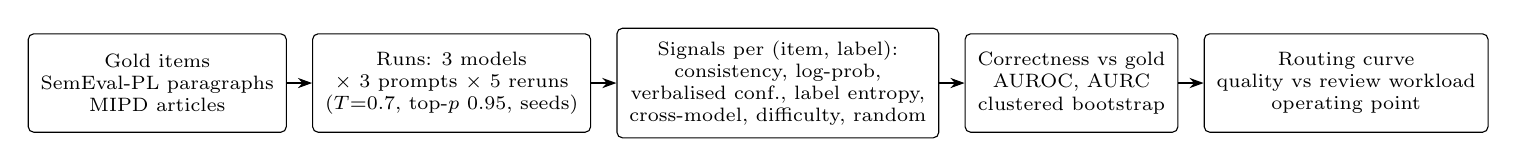
\begin{tikzpicture}[
    node distance=0.32cm,
    box/.style={
        draw,
        rounded corners=2pt,
        align=center,
        font=\scriptsize,
        inner sep=4.5pt,
        minimum height=1.25cm
    },
    arrow/.style={-{Stealth[length=1.8mm, width=1.3mm]}, thin}
]
\node[box] (n1) {Gold items\\SemEval-PL paragraphs\\MIPD articles};
\node[box, right=of n1] (n2) {Runs: 3 models\\$\times$ 3 prompts $\times$ 5 reruns\\($T$=0.7, top-$p$ 0.95, seeds)};
\node[box, right=of n2] (n3) {Signals per (item, label):\\consistency, log-prob,\\verbalised conf., label entropy,\\cross-model, difficulty, random};
\node[box, right=of n3] (n4) {Correctness vs gold\\AUROC, AURC\\clustered bootstrap};
\node[box, right=of n4] (n5) {Routing curve\\quality vs review workload \\operating point};

\draw[arrow] (n1) -- (n2);
\draw[arrow] (n2) -- (n3);
\draw[arrow] (n3) -- (n4);
\draw[arrow] (n4) -- (n5);
\end{tikzpicture}
\caption{Five stage experimental pipeline.}
\label{fig:pipeline}
\end{figure*}

\subsection{Experimental setup}

We compare three instruction-tuned models: Bielik-11B-v3.0,
PLLuM-12B and Gemma-3-12B-it. Evaluation uses the Polish
SemEval-2023 development set (800 paragraphs from 49 articles)
and a stratified sample of 1,000 MIPD test articles.
Separate calibration sets comprise 200 SemEval training paragraphs,
sampled by source article, and 200 MIPD validation articles.
They are used for prompt verification and threshold selection.

Each model uses three prompts: technique names only, names with
official annotation definitions (following the MIPD guidelines
for manipulation techniques~\cite{mipd-2024}), and a paraphrased
annotation rubric.
For each prompt, we collect five stochastic outputs at temperature
0.7 and top-$p$ 0.95, plus one greedy reference output.
Each output contains a binary decision and verbalised confidence
for every technique. Sampling parameters and seeds are fixed
across configurations. Sampling variability is analysed within
prompts, and prompt sensitivity across prompts.

\subsection{Confidence signals}

For each item--label pair, the predicted label is the majority
decision across five reruns within a prompt. Self-consistency
is the fraction of reruns supporting that decision.
We compare it with decision-token log-probability, mean verbalised
confidence, entropy across prompt variants, cross-model agreement,
a label-specific correctness prior estimated on calibration data,
and random routing. All signals will score the correctness of the same final majority-vote decision. Aggregation rules will be established
on calibration data before held-out evaluation.
Log-probabilities refer only to binary label decisions,
excluding confidence scores and JSON formatting.

\subsection{Evaluation and routing}

Annotation quality is measured using macro-F1, micro-F1 and per-label
F1. We assess whether consistency predicts correctness using
Spearman correlation between item-level consistency and F1,
and the area under the receiver operating characteristic curve
(AUROC) for individual label decisions. Results are reported per model, dataset and label. We analyse positive and negative gold labels separately, and assess errors among accepted positive and negative predictions to expose class-imbalance effects.
Item-level F1 is defined as 1 when both predicted and gold label
sets are empty.

We also report the area under the risk--coverage curve, where risk
is the error rate among accepted decisions and coverage is their
share of all decisions. Expected calibration error is computed
for signals expressed as correctness probabilities.
We estimate 95\% confidence intervals using 1,000 bootstrap
resamples at the source-article level.

Routing accepts high-confidence model decisions and replaces
deferred decisions with gold labels, simulating ideal correction
rather than measured human review. We plot hybrid macro-F1 against decision coverage. For workload estimates, an item requires review if any of its labels is deferred.

These settings and routing thresholds will be fixed before
held-out evaluation. Deliverables include the signal comparison,
routing curves and a reproducible experiment.


\section{Contributions and AI declaration}
Table~\ref{tab:contrib} presents the contributions of each team member
during this phase of the project.

\noindent
{\small
\setlength{\tabcolsep}{3pt}
\renewcommand{\arraystretch}{1.12}
\begin{center}
\begin{tabular}{@{}l
  >{\raggedright\arraybackslash}p{0.55\columnwidth}@{}}
\toprule
\textbf{Author} & \textbf{Contribution} \\
\midrule
Mikołaj Twardowski & Introduction, related work, state-of-the-art, and table comparing papers (8h)\\
Aleksandra Idczak & Datasets and their status, initial EDA, and data statement (8h)\\
Kacper Wnęk & Solution concept, experimental plan, and experiment pipeline diagram (8h)\\
\bottomrule
\end{tabular}
\captionof{table}{Contribution table}
\label{tab:contrib}
\end{center}
}


LLMs were and will be used for literature searching and for helping understand information, results and metodology from these scientific articles. LLMs were used to help perform data aggregations (label distribution) and will be used for helping with generation of code. LLMs helped organize this latex report - mostly for shortening the text, for structuring the tables, and for some language formulation.
The authors are responsible for verifying all claims, references, and methodological choices.


\bibliographystyle{unsrt}
\bibliography{overleaf/references}


\appendix
\onecolumn

\section{Additional Tables}

% ------------------------------------------------
% TABLE 1: MIPD label distribution
% ------------------------------------------------

\begin{center}
\small
\renewcommand{\arraystretch}{1.05}
\begin{tabularx}{\textwidth}{@{}
>{\raggedright\arraybackslash}p{0.35\textwidth}
>{\raggedright\arraybackslash}X
>{\raggedright\arraybackslash}X
>{\raggedright\arraybackslash}X
@{}}
\toprule
Label & train & val & test \\
\midrule
Exaggeration & 1514 (14.1\%) & 405 (13.1\%) & 234 (15.4\%) \\
Cherry picking & 1082 (10.1\%) & 295 (9.6\%) & 149 (9.8\%) \\
Reference error & 762 (7.1\%) & 227 (7.4\%) & 119 (7.8\%) \\
Emotional content & 635 (5.9\%) & 182 (5.9\%) & 92 (6.0\%) \\
False cause & 627 (5.8\%) & 193 (6.3\%) & 95 (6.2\%) \\
Strawman & 321 (3.0\%) & 76 (2.5\%) & 37 (2.4\%) \\
Anecdote & 310 (2.9\%) & 88 (2.9\%) & 44 (2.9\%) \\
Whataboutism & 307 (2.9\%) & 82 (2.7\%) & 37 (2.4\%) \\
Misleading clickbait & 123 (1.1\%) & 41 (1.3\%) & 13 (0.9\%) \\
Leading questions & 92 (0.9\%) & 20 (0.6\%) & 15 (1.0\%) \\
Quote mining & 88 (0.8\%) & 23 (0.7\%) & 14 (0.9\%) \\
\midrule
(no label) & 8146 (75.8\%) & 2360 (76.5\%) & 1148 (75.5\%) \\
\textit{Total articles} & \textit{10749} & \textit{3086} & \textit{121} \\
\bottomrule
\end{tabularx}

\captionof{table}{MIPD: label distribution per split. Shares add up to more than 100\% because an article can carry several labels.}
\label{tab:mipd-labels}
\end{center}

\vspace{-2cm}

% ------------------------------------------------
% TABLE 2: SemEval label distribution
% ------------------------------------------------

\begin{center}
\small
\renewcommand{\arraystretch}{1.0}
\begin{tabularx}{\textwidth}{@{}
>{\raggedright\arraybackslash}p{0.52\textwidth}
>{\raggedright\arraybackslash}X
>{\raggedright\arraybackslash}X
@{}}
\toprule
Label & train & dev \\
\midrule
Name Calling or Labeling & 475 (20.6\%) & 111 (13.9\%) \\
Loaded Language & 310 (13.4\%) & 93 (11.6\%) \\
Doubt & 295 (12.8\%) & 96 (12.0\%) \\
Questioning the Reputation & 164 (7.1\%) & 57 (7.1\%) \\
Appeal to Hypocrisy & 162 (7.0\%) & 76 (9.5\%) \\
Exaggeration or Minimisation & 111 (4.8\%) & 40 (5.0\%) \\
Appeal to Fear or Prejudice & 108 (4.7\%) & 36 (4.5\%) \\
Appeal to Values & 101 (4.4\%) & 50 (6.2\%) \\
Guilt by Association & 94 (4.1\%) & 30 (3.8\%) \\
Flag Waving & 68 (2.9\%) & 28 (3.5\%) \\
Conversation Killer & 50 (2.2\%) & 40 (5.0\%) \\
Appeal to Authority & 41 (1.8\%) & 40 (5.0\%) \\
Obfuscation or Vagueness or Confusion & 36 (1.6\%) & 11 (1.4\%) \\
Slogans & 36 (1.6\%) & 7 (0.9\%) \\
Appeal to Popularity & 30 (1.3\%) & 22 (2.8\%) \\
Consequential Oversimplification & 24 (1.0\%) & 8 (1.0\%) \\
Straw Man & 15 (0.6\%) & 3 (0.4\%) \\
Appeal to Time & 14 (0.6\%) & 5 (0.6\%) \\
Repetition & 13 (0.6\%) & 10 (1.2\%) \\
False Dilemma or No Choice & 12 (0.5\%) & 8 (1.0\%) \\
Red Herring & 12 (0.5\%) & 7 (0.9\%) \\
Causal Oversimplification & 12 (0.5\%) & 5 (0.6\%) \\
Whataboutism & 8 (0.3\%) & 3 (0.4\%) \\
\midrule
(no label) & 1078 (46.7\%) & 377 (47.1\%) \\
\textit{Total paragraphs} & \textit{2310} & \textit{800} \\
\bottomrule
\end{tabularx}

\captionof{table}{SemEval-2023 Task 3 (Polish): label distribution per split. Shares add up to more than 100\% because a paragraph can carry several labels.}
\label{tab:semeval-labels}
\end{center}

\vspace{1em}

% ------------------------------------------------
% TABLE 3: Project plan
% ------------------------------------------------

\begin{center}
\footnotesize
\renewcommand{\arraystretch}{1.1}
\begin{tabularx}{\textwidth}{@{}
l
>{\raggedright\arraybackslash}X
>{\raggedright\arraybackslash}X
>{\raggedright\arraybackslash}X
@{}}
\toprule
\textbf{Week} & \textbf{Aleksandra} & \textbf{Mikołaj} & \textbf{Kacper} \\
\midrule
4--11.11 & EDA of both datasets & Repository and model access & Prompt variants and first end-to-end PoC run \\
11--18.11 & Dataset comparison; mid-term video & Rerun logging; mid-term video & Mid-term slides and video \\
\midrule
18--25.11 & Prepare Q\&A presentation & Runtime and memory measurements & Classical baseline\\
25.11--2.12 & PoC code and EDA section of the report & PoC code and literature section of the report & PoC code and write README \\
\midrule
2--9.12 & Evaluation code for consistency and correctness & Start full model reruns & Extract log-probability and verbalised-confidence signals \\
9--16.12 & First AUC results with confidence intervals & Finish model reruns; reproducibility: seeds, configs and commands & Random-routing baseline and signal comparison; first routing curve \\
16--23.12 & Per-model and per-label analysis; error analysis; report draft & Fix any failed runs; final code clean-up & Final routing curve and operating point; results and discussion sections \\
24.12--5.01 & \multicolumn{3}{c}{\textit{Winter break}} \\
6--13.01 & Final video and final report polishing & Final video and final report polishing & Final video and final report polishing \\
\bottomrule
\end{tabularx}

\captionof{table}{Week-by-week project plan showing the tasks owned by each team member.}
\label{tab:project-plan}
\end{center}


\end{document}